% declare our document type
\documentclass[12pt]{extarticle}

%%%%%%%% PACKAGES NEEDED FOR THIS DOCUMENT

%allow us to create diagrams
\usepackage{tikz}
%used for color
\usepackage{xcolor}
% allow us to put pictures in the document
\usepackage{graphicx}
% this line lets us use larger fonts
\usepackage{extsizes}
% this allows us to create "slides" in the document
\usepackage[many]{tcolorbox}
% this line lets us caption images inside the "slides"
% this is neccesary since the slide doesn't allow the use of
% \figure{} inside
\usepackage{caption}
% sets up tables so that they autoformat
\usepackage{array}
\newcolumntype{L}[1]{>{\raggedright\let\newline\\\arraybackslash\hspace{0pt}}m{#1}}
\newcolumntype{C}[1]{>{\centering\let\newline\\\arraybackslash\hspace{0pt}}m{#1}}
\newcolumntype{R}[1]{>{\raggedleft\let\newline\\\arraybackslash\hspace{0pt}}m{#1}}
% allows use of courier font
\usepackage{courier}
% make the table of contents links like people are used to
% the hidelinks parts hides link outlines
\usepackage[hidelinks]{hyperref}
% resize the margins
\usepackage[margin=1in]{geometry}
% specially resizable tables
\usepackage{tabularx}
% use utf8 encoding
\usepackage[utf8]{inputenc}
% one of the other packages complained until I put this here
\usepackage[english]{babel}
% allow citations
\usepackage{cite}
% code listings
\usepackage{listings}
\lstset{frame=tb,
	language=Python,
	aboveskip=3mm,
	belowskip=3mm,
	showstringspaces=false,
	columns=flexible,
	basicstyle={\small\ttfamily},
	numbers=none,
	numberstyle=\tiny\color{gray},
	keywordstyle=\color{blue},
	commentstyle=\color{green},
	stringstyle=\color{red},
	breaklines=true,
	breakatwhitespace=true,
	tabsize=3
}
% fix single quote in listings
\usepackage{textcomp}
\usepackage{filecontents}
%\usepackage[noadjust]{cite}
\usepackage{graphicx}
\usepackage{hyperref}
\usepackage{forest,kantlipsum}
\usepackage{float}
\usepackage{etoolbox}
\usepackage{url}
\usepackage{cleveref}
\usepackage{xcolor}
\usepackage[labelfont=bf]{caption}

%%%%%%%%%%% CUSTOM ENVIRONMENT SETUP

% declare a typesetting environment for code/emphasis
\newcommand{\code}[1]{\texttt{\bfseries#1}}
\newenvironment{codeblock}{\bfseries\texttt\bgroup}{\egroup\par}
% better declaration of font environment
%\DeclareTextFontCommand{\codetext}[1]{\code{#1}}
% declare a large font environment for use in the ''slides''
\newcommand{\instruction}[1]{\Large{#1}}
% font environment again
%\DeclareTextFontCommand{\instruction}{\instructionfont}
\newenvironment{instructionblock}{\Large\bgroup}{\egroup}
% declare a ''slide'' text box for use in the document
% the slide is a numbered \section{}
\newtcolorbox[auto counter]{slide}[3][]{%
	colback=brown!5!white,colframe=brown!80!gray,height=3.72in,
	title={\addcontentsline{toc}{section}{\thetcbcounter ~~ #2}\bf\Large\thetcbcounter ~ #2\hfill #3 \label{slide \thetcbcounter}\setcounter{section}{\thetcbcounter}}}
% declare a ''subslide'' text box for use in the document
% the subslide is a numbered \subsection{}
\newtcolorbox[auto counter,number within=section]{subslide}[3][]{%
	colback=brown!5!white,colframe=brown!80!gray,height=3.72in,
	title={\addcontentsline{toc}{subsection}{\thetcbcounter ~~ #2}\bf\Large\thetcbcounter ~ #2\hfill #3 \label{slide \thetcbcounter}}}
\renewcommand{\labelitemii}{$\circ$}
\lstset{basicstyle=\ttfamily,keywordstyle=\bfseries\color{blue!80!black},identifierstyle=\bfseries,stringstyle=\color{red},showstringspaces=false,commentstyle=\itshape\color{green!40!black},upquote=true}

% The following code is courtesy of Chris Ocker and the susequent code used for automatic Beamer slide linking
% My Environments (keep these)
\newcommand{\ben}{\begin{enumerate}}
\newcommand{\een}{\end{enumerate}}
\newcommand{\bi}{\begin{itemize}}
\newcommand{\ei}{\end{itemize}}
\usepackage{titling}
\newcounter{questionEnumerate}
\newcounter{next}
\setcounter{next}{2}
\newcounter{prev}
\setcounter{prev}{0}
\usepackage{hyperref}
\hypersetup{
	colorlinks=true,
	linkcolor=blue,
	filecolor=blue,      
	urlcolor=blue,
	citecolor=blue,
}


%\setlength{\arrayrulewidth}{1mm}
%\setlength{\tabcolsep}{18pt}
%\renewcommand{\arraystretch}{2.5}



%%%%%%%%% SET UP OUR TITLE PAGE

\begin{document}
\title{ICS Firewall Configuration Through Vulnerability Assessment}
\author{Matt Kirkland}
\date{\today \\ \hyperref[changelog]{Version 1.0}} %\today
\renewcommand{\abstractname}{Summary}
\begin{titlepage}
\maketitle
\pagenumbering{gobble}
\begin{center}

\includegraphics[scale=.5]{UofI}

\large{CS 536: Advanced Information Assurance}

\vskip 40pt

\textbf{Abstract}\\
The purpose of this document is to introduce basic control system and network configuration. A simplified vulnerability assessment is performed on a small, virtualized water treatment ICS network. The students will learn the basics of hardening and ICS network using best practices taken from NIST SP 800-82.
\end{center}


\vfill
\begin{center}

\includegraphics[scale=.5]{cc}\\
This work is licensed under a \href{https://creativecommons.org/licenses/by/2.0/}{Creative Commons Attribution 2.0 Generic License}.
\vskip 10pt
\end{center}

\end{titlepage}

%%%%%%%%%% TABLE OF CONTENTS

\pagebreak
\tableofcontents

%%%%%%%%%%%%%%%%%%%%%%%%%%%%%%%%%%%%%%%%%%%%%%%%%
%%%%%%    BEGINNING OF ACTUAL DOCUMENT
%%%%%%%%%%%%%%%%%%%%%%%%%%%%%%%%%%%%%%%%%%%%%%%%%

\pagebreak
\pagenumbering{arabic}
\setcounter{section}{1}



%-----------------------------------------------------------------------------------------------------------------------------------------------------------------------------------------------------------------%

	\pagebreak
	\setcounter{section}{1}
	\begin{slide}{Objectives of this Tutorial}{\hyperref[slide \thenext]{\textgreater}}
		\begin{instructionblock}
				\bi 
					\item Introduce basic ICS network configuration
					\item Understand the outline of a vulnerability assessment
					\item Perform a simplified,mock vulnerability assessment
					\item Apply firewall configurations as recommended in NIST SP800-82
				\ei
		\end{instructionblock}
	\end{slide}
	
	
%-----------------------------------------------------------------------------------------------------------------------------------------------------------------------------------------------------------------%	
	
	
	\pagebreak
	\stepcounter{next}
	\stepcounter{prev}	
	\begin{slide}{Required Background}{\hyperref[slide \theprev]{\textless}\hyperref[slide \thenext]{\textgreater}}
		%\vskip 10 pt
		\begin{instructionblock}
			\bi
				\item Ability to work with virtual machines (i.e. Virtual Box, VMware, etc.)
				\item Basic understanding of ICS and MODBUS protocol
				\item Knowledge of introductory Cybersecurity/information assurance material
				\item Familiarity with networking and firewall appliances
			\ei
		\end{instructionblock}
	\end{slide}
	
	\pagebreak
	


%-----------------------------------------------------------------------------------------------------------------------------------------------------------------------------------------------------------------%

\pagebreak
\stepcounter{next}
\stepcounter{prev}
\begin{slide}{Info: Review of Previous Tutorial}{\hyperref[slide \theprev]{\textless}\hyperref[slide \thenext]{\textgreater}}
	%\vskip 10 pt
	\begin{instructionblock}
		Last time we looked at:
		\bi
			\item An introduction to Industrial Control Systems
			\item What is a PLC? How does Ladder Logic work?
			\item The MODBUS industrial protocol
			\item Injection attacks on PLCs with PyModbus
		\ei
	\end{instructionblock}
\end{slide}
\textit{Duration: 1 minute}
\vfill
\noindent
%Place information here
\pagebreak

%-----------------------------------------------------------------------------------------------------------------------------------------------------------------------------------------------------------------%

\pagebreak
\stepcounter{next}
\stepcounter{prev}
\begin{slide}{Info: The Basic ICS Network}{\hyperref[slide \theprev]{\textless}\hyperref[slide \thenext]{\textgreater}}
	%\vskip 10 pt
	\vspace{-.75cm}
	\begin{figure}[H]
		\centering
		\includegraphics[width=10.4cm]{"Figures/vWaterLab-Network Diagram".png}
		\caption{Sample ICS network configuration}
	\end{figure}
\end{slide}
\textit{Duration: 1 minute}
\vfill
\noindent
The above model is based on the 4-layer  ANSI/ISA-99 reference model for ICS:
\bi
	\item \textbf{Enterprise Network:} While not directly part of the actual ICS network, almost all ICS networks are connected to an Enterprise network. The Enterpise network consists of traditional IT infrastructure. While there may be legitimate reasons for this network to connect to the ICS, they should be rare. Many attacks on the ICS networks come from this area.
	\item \textbf{Supervisory Network:} Composes of machines that control the entire process of the ICS (ex. SCADA) or machines that need access to information provided at this level (ex. Historian, Engineering Workstation, etc.).
	\item \textbf{Control Network:} Made up of localized control devices, or rather devices that automate part of the industrial process (ex. PLCs, RTUs, Smart Relays, etc.). It is not uncommon for one of these devices to control other control devices in a master/slave relationship. However, these devices typically are directly wired to field devices that make up the "I/O Network".
	\item \textbf{I/O Layer:} A layer that consists of devices that gather information from the field (i.e. sensing) or they manipulate the physical world (i.e. actuation). A sensor is a field device that reads information about the real world (ex. thermostat or water level sensor). An actuator is a field device that acts out or makes changes to the physical world (ex. pump or motor).
\ei
\pagebreak

%-----------------------------------------------------------------------------------------------------------------------------------------------------------------------------------------------------------------%


\pagebreak
\stepcounter{next}
\stepcounter{prev}
\begin{slide}{Info: PLC \& SCADA Review}{\hyperref[slide \theprev]{\textless}\hyperref[slide \thenext]{\textgreater}}
	%\vskip 10 pt
	\begin{instructionblock}
		Supervisory Control \& Data Acquisition (SCADA)
		\bi
			\item Controls the entire process
			\item Often has a web interface (HMI)
			\item Manages PLCs to control the process
		\ei
		Programmable Logic Controller
		\bi
			\item Controls a subset of the process
			\item Often directly connected to I/O
			\item Takes orders from the SCADA or other PLCs
		\ei
	\end{instructionblock}
\end{slide}
\textit{Duration: 1 minute}
\vfill
\noindent
\textbf{Supervisory Control and Data Acquisition (SCADA)}\\
Inductive Automation\cite{inductAuto} defines a SCADA as a system that performs the following functions to an industrial process:
\bi
	\item "Control industrial processes locally or at remote locations"
	\item "Monitor, gather, and process real-time data"
	\item "Directly interact with devices such as sensors, valves, pumps, motors, and more through human-machine interface (HMI) software"
	\item "Record events into a log file"
\ei
The SCADA can do these things because other automation devices like PLCs report relevant information to them from the actual I/O devices. For example, a thermostat reports to the PLC it's current value. The PLC interprets this information as a temperature for a room. The PLC can then forward this information to the SCADA in a useful manner. \\\\
\textbf{Programmable Logic Controller (PLC)}\\
A PLC is a type of type of local control device. As seen in the previous example, it is often directly connected to I/O and interprets this information in a way that is understandable for the SCADA. Both the SCADA and PLC use similar ICS network protocols (ex. MODBUS). 
\pagebreak
%-----------------------------------------------------------------------------------------------------------------------------------------------------------------------------------------------------------------%

\pagebreak
\stepcounter{next}
\stepcounter{prev}
\begin{slide}{Info: Vulnerability Assessment}{\hyperref[slide \theprev]{\textless}\hyperref[slide \thenext]{\textgreater}}
	%\vskip 10 pt
	\begin{instructionblock}
		\bi
			\item[]\textbf{Def:} A form of risk assessment that focuses on security
			\item[]\textbf{Goal:} Vulnerability Assessment vs. Penetration test
			\item[]\textbf{Forms:} Theoretical and Physical tests (online and offline)
		\ei
		\begin{figure}[H]
			\centering
			\includegraphics[width=9cm]{"Figures/3phaseVulnAssess".png}
		\end{figure}
	\end{instructionblock}
\end{slide}
\textit{Duration: 5 minutes}
\vfill
\noindent
\textbf{Vulnerability Assessment}\\
Knapp et al. explain that, "Vulnerabilities can be found either by evaluating the system in the form of an assessment, or by attempting to attack the system in a manner consistent with what a hacker or external threat may do..."\cite{KnappLangill}. The former is a Vulnerability Assessment and the former is a Penetration test.\\
There are two kinds of Vulnerability Assessments: Physical and Theoretical. Theoretical involves no actual contact with the system to be tested. Physical involves contact and can be further sub-divided into two categories. Physical Assessments can further take on the form of an "online" or "offline". An online assessment utilizes the actual hardware of the system in question. This is very dangerous, because the assessment could upset the system it intends to protect. Offline involves testing a subset of the total system (usually not connected).\cite{KnappLangill}
\pagebreak

%-----------------------------------------------------------------------------------------------------------------------------------------------------------------------------------------------------------------%

\pagebreak
\stepcounter{next}
\stepcounter{prev}
\begin{slide}{Info: General V.A. Procedure}{\hyperref[slide \theprev]{\textless}\hyperref[slide \thenext]{\textgreater}}
	%\vskip 10 pt
	\begin{instructionblock}
		\ben
		\item System characterization
		\item Threat identification
		\item Vulnerability identification
		\item Risk Classification and Ranking
		\item Risk Reduction and Mitigation
		\een
	\end{instructionblock}
\end{slide}
\textit{Duration: 1 minute}
\vfill
\noindent
\textbf{System characterization}\\
Identify all of the resources that are within and outside the scope of the assessment. Data collection is performed. Network, vulnerability, traffic scanning are common.\cite{KnappLangill} \\\\
\textbf{Threat identification}\\
These phase consists of (1) Identification of threat sources (ex. customer, supplier, national state, etc.). (2) Identification of threat vectors (i.e. the means of impact by the threat actor) (3) Development of attacks possible to the threat actor via aforementioned vectors. \cite{KnappLangill}\\\\
\textbf{Vulnerability identification}\\
This is the part of the assessment where security weaknesses, or areas that are suceptable to leveraging of a threat actor, are identified. This phase relies heavily on automated tools (ex. OpenVAS) to provide these details. \cite{KnappLangill}\\\\
\textbf{Risk Classification and Ranking}\\
This phase attempts to compare risks identified in the assessment and provide valuable metrics like: consequence and likelihood. Microsoft developed a model that aids in developing these metrics called DREAD; It is commonly used in Vulnerability Assessment. \cite{KnappLangill}\\\\
\textbf{Risk Reduction and Mitigation}\\
This phase focuses on using the information gathered thus far to plan for improvements to mitigate the highest risk scenarios and reduce the overall cyber risk of the system. \cite{KnappLangill}
\pagebreak

%-----------------------------------------------------------------------------------------------------------------------------------------------------------------------------------------------------------------%


\pagebreak
\stepcounter{next}
\stepcounter{prev}
\begin{slide}{Info: Scenario}{\hyperref[slide \theprev]{\textless}\hyperref[slide \thenext]{\textgreater}}
	%\vskip 10 pt
	\begin{instructionblock}
		You have been contracted by WaterTank LLC to perform a vulnerability assessment of their ICS systems. They would like you to perform an offline assessment on their older equipment they used to use for water disinfection. They are a relatively new startup and have just begun staffing full-time cybersecurity personnel. Your job is to give a baseline of their security posture based on your findings on this small testbed.
	\end{instructionblock}
\end{slide}
\vfill
\noindent
%Place information here
\pagebreak

%-----------------------------------------------------------------------------------------------------------------------------------------------------------------------------------------------------------------%

\pagebreak
\stepcounter{next}
\stepcounter{prev}
\begin{slide}{Info: Network Scans Guidelines for ICS}{\hyperref[slide \theprev]{\textless}\hyperref[slide \thenext]{\textgreater}}
	%\vskip 10 pt
	\begin{instructionblock}
		\bi
		\item Test scans methods prior to use on a live system
		\item Avoid "high interaction" scans
		\item Low interaction methods: Passive listening, IDS \& Firewall review, print local route and arp tables, etc.
		\ei
	\end{instructionblock}
\end{slide}
\vfill
\noindent
%Place information here
\pagebreak

%-----------------------------------------------------------------------------------------------------------------------------------------------------------------------------------------------------------------%

\pagebreak
\stepcounter{next}
\stepcounter{prev}
\begin{slide}{Task: Scan the ICS Network}{\hyperref[slide \theprev]{\textless}\hyperref[slide \thenext]{\textgreater}}
	%\vskip 10 pt
	\begin{instructionblock}
		We will start by scanning the network to identify our network assets. Use nmap to accomplish this end.\\\\
		\textbf{WARNING:} Please refrain from using aggressive scans!
 	\end{instructionblock}
\end{slide}
\textit{Duration: 5 minutes}
\vfill
\noindent
Host discovery
\ben
	\item Log on to the Kali box
	\item Open the terminal window
	\item Run a scan on the network: \textit{nmap -sn 192.168.10.0/24}
	\item Review your findings and build a network map
	\item Nmap should have found 4 machines:
	\bi
		\item 192.168.10.1
		\item 192.168.10.22
		\item 192.168.10.25
		\item 192.168.10.29 (Kali Linux)
	\ei
\een
\pagebreak

%-----------------------------------------------------------------------------------------------------------------------------------------------------------------------------------------------------------------%

\pagebreak
\stepcounter{next}
\stepcounter{prev}
\begin{slide}{Info: MODBUS Review}{\hyperref[slide \theprev]{\textless}\hyperref[slide \thenext]{\textgreater}}
	%\vskip 10 pt
	\begin{instructionblock}
		MODBUS
		\bi
			\item A standard application layer protocol commonly used in ICS environments for communication between controllers (ex. PLC,HMI,SCADA,etc.)
			\item Operations: Reading and writing to coils and registers
			\item Commonly on Port 502 (new \href{modbus.org/docs/Modbus-SecurityPR-10-2018.pdf}{MODBUS Security} uses 802)
			\item Many variants: serial, TCP/IP, MODBUS PLUS, etc.
		\ei
	\end{instructionblock}
\end{slide}
\vfill
\noindent
%Place information here
For more information please check: \url{http://www.modbus.org/docs/Modbus_Application_Protocol_V1_1b3.pdf}
\pagebreak

%-----------------------------------------------------------------------------------------------------------------------------------------------------------------------------------------------------------------%

\pagebreak
\stepcounter{next}
\stepcounter{prev}
\begin{slide}{Challenge: Passive Service Identification}{\hyperref[slide \theprev]{\textless}\hyperref[slide \thenext]{\textgreater}}
	%\vskip 10 pt
	\begin{instructionblock}
		Identify the ICS components detected in the previous scan. Please keep the following in mind:
		\bi
			\item Do NOT use aggressive methods (i.e. Nmap port scans).
			\item Wireshark is HIGHLY recommended
			\item Passive methods only!
		\ei
	\end{instructionblock}
\end{slide}
\textit{Duration: 20 minutes}
\vfill
\noindent
%Place information here
\pagebreak
%-----------------------------------------------------------------------------------------------------------------------------------------------------------------------------------------------------------------%

\pagebreak
\stepcounter{next}
\stepcounter{prev}
\begin{slide}{Discussion: Identify High-value Assets}{\hyperref[slide \theprev]{\textless}\hyperref[slide \thenext]{\textgreater}}
	%\vskip 10 pt
	\begin{instructionblock}
		Determine what the most high-value assets are given this information:
		\bi
			\item Backup equipment: PLC A, SCADA
			\item REMEMBER: SCADA controls the whole process
		\ei 
	\end{instructionblock}
\end{slide}
\textit{Duration: 5 minutes}
\vfill
\noindent
Determine the high-value assets based on equipment available and the priority of each machine.
\pagebreak
%-----------------------------------------------------------------------------------------------------------------------------------------------------------------------------------------------------------------%

\pagebreak
\stepcounter{next}
\stepcounter{prev}
\begin{slide}{Task: Examine the Firewall Rules}{\hyperref[slide \theprev]{\textless}\hyperref[slide \thenext]{\textgreater}}
	%\vskip 10 pt
	\begin{instructionblock}
		Determine current rules and how the ICS network is configured using the pfSense web interface.
		\ben
			\item Log-on to the Kali machine
			\item Enter \textit{192.168.10.1} into the browser
			\item Log-on to the pfSense box and examine the firewall rules
		\een
	\end{instructionblock}
\end{slide}
\textit{Duration: 10 minutes}
\vfill
\noindent
%Place information here
\pagebreak
%-----------------------------------------------------------------------------------------------------------------------------------------------------------------------------------------------------------------%

\pagebreak
\stepcounter{next}
\stepcounter{prev}
\begin{slide}{Challenge: MODBUS Injection Attack}{\hyperref[slide \theprev]{\textless}\hyperref[slide \thenext]{\textgreater}}
	%\vskip 10 pt
	\begin{instructionblock}
		Perform a MODBUS injection attack against the outbound pump. Check on the HMI to ensure the attack is successful. 
	\end{instructionblock}
\end{slide}
\textit{Duration: 15 minutes}
\vfill
\noindent
%Information here!
\pagebreak
%-----------------------------------------------------------------------------------------------------------------------------------------------------------------------------------------------------------------%

\pagebreak
\stepcounter{next}
\stepcounter{prev}
\begin{slide}{Discussion: Mitigate the attack}{\hyperref[slide \theprev]{\textless}\hyperref[slide \thenext]{\textgreater}}
	%\vskip 10 pt
	\begin{instructionblock}
		How would you use the firewall to block this attack script? Ensure that your proposed methods do NOT block basic functionality of the ICS system. What considerations would you employ?
	\end{instructionblock}
\end{slide}
\textit{Duration: 25 minutes}
\vfill
\noindent
%Place information here
\pagebreak
%-----------------------------------------------------------------------------------------------------------------------------------------------------------------------------------------------------------------%

\pagebreak
\stepcounter{next}
\stepcounter{prev}
\begin{slide}{Info: Recommended Best Practices}{\hyperref[slide \theprev]{\textless}\hyperref[slide \thenext]{\textgreater}}
	%\vskip 10 pt
	\begin{instructionblock}
		NIST SP800-82: ICS Firewalls
		\bi
			\item Allow ONLY specified communications in the ICS network
			\item Prohibit insecure/unnecessary protocols (ex. email)
			\item NO unacceptable delay to ICS communications
		\ei
		NIST SP800-82: ICS Network Configuration
		\bi
			\item At least one firewall between the Enterprise \& ICS networks
			\item Three-zone separation with at least one DMZ
			\item No dual NIC machines (other than firewalls)
		\ei
	\end{instructionblock}
\end{slide}
\textit{Duration: 3 minutes}
\vfill
\noindent
\textbf{NIST SP800-82}\\
"NIST Special Publications 800-82: Guide to Industrial Control Systems (ICS) Security"\cite{Stouffer2014}  outlines best practices for control system security. It cites various general network and firewall configurations guidelines. Specifically, this author cites some of these important standards. In general, apply the principle of least privilege. Only allow necessary communications in and out of the ICS network. This also applies to protocols allowed into each ICS zone. It is important to remember that these security configurations should not result in performance decreases that render the industrial process less effective.\\
When it comes to general network configuration, implementation of network separation is one of the key concepts. In general, a Demilitarized Zone (DMZ) should separate the ICS from external connections (usually the Enterprise Network). Separating the ICS network into security zones based on purpose may allow for the usage of more powerful firewall filtering and greater defense in depth. Avoid technologies that subvert this sort of configuration, such as machines with multiple network interfaces.\cite{Stouffer2014} 
\pagebreak

%-----------------------------------------------------------------------------------------------------------------------------------------------------------------------------------------------------------------%

\pagebreak
\stepcounter{next}
\stepcounter{prev}
\begin{slide}{Info: Vulnerability Assessment Report}{\hyperref[slide \theprev]{\textless}\hyperref[slide \thenext]{\textgreater}}
	%\vskip 10 pt
	\begin{instructionblock}
		A report should contain:
		\bi
			\item Scope of assessment and purpose
			\item List of tests performed and their results
			\item A listing of vulnerabilities found
			\item Suggested mitigations based on potential impact
		\ei
	\end{instructionblock}
\end{slide}
\textit{Duration: 2 minutes}
\vfill
\noindent
%Place information here
The University of Iowa has a \href{https://itsecurity.uiowa.edu/sites/itsecurity.uiowa.edu/files/sampleriskassessmentreport.pdf}{sample security risk assessment report} that represents what the reports should look like.
\pagebreak

%-----------------------------------------------------------------------------------------------------------------------------------------------------------------------------------------------------------------%

\pagebreak
\stepcounter{next}
\stepcounter{prev}
\begin{slide}{Info: CVSS and Risk Management}{\hyperref[slide \theprev]{\textless}\hyperref[slide \thenext]{\textgreater}}
	%\vskip 10 pt
	\begin{instructionblock}
	\bi
		\item Common Vulnerability Scoring System
		\item CVSS combined with Asset priority list
		\item Risk management in terms of most effective for the cost
	\ei
	\end{instructionblock}
\end{slide}
\textit{Duration: 5 minutes}
\vfill
\noindent
\textbf{Common Vulnerability Scoring System (CVSS)}\\
The CVSS is globally recognized standard that is used for determining the total consequence involved with a given vulnerability. This tool (and others like it) is used in the "Vulnerability identification" phase of Vulnerability Assessment. A variety of metrics are evaluated and fall into the following categories: (1) Base - the base unmitigated risk of given no mitigations are implemented. (2) Temporal - a refinement of the base metrics based on time. (3) Environment - a refinement of the base metrics based on the particular environment they are located. \cite{KnappLangill}\\\\
\textbf{Asset Priority List}\\
This should detail the highest priority assets of the industrial process. It is important to utilize cross-functional teams to develop accurate rankings of assets.
\pagebreak

%-----------------------------------------------------------------------------------------------------------------------------------------------------------------------------------------------------------------%

\pagebreak
\stepcounter{next}
\stepcounter{prev}
\begin{slide}{Info: Conclusion}{\hyperref[slide \theprev]{\textless}\hyperref[slide \thenext]{\textgreater}}
	%\vskip 10 pt
	\begin{instructionblock}
		\bi
			\item We reviewed network infrastructure of an ICS
			\item Described common ICS components
			\item Talked about vulnerability assessments
			\item Performed a toy assessment
			\item Discussed how risk management plays a role in mitigation development
		\ei
	\end{instructionblock}
\end{slide}
\textit{Duration: 3 minutes}
\vfill
\noindent
%Place information here
\pagebreak

%-----------------------------------------------------------------------------------------------------------------------------------------------------------------------------------------------------------------%

\pagebreak
\stepcounter{next}
\stepcounter{prev}
\begin{slide}{Appendix}{\hyperref[slide \theprev]{\textless}}
	\begin{instructionblock}
		\ben
		\item Solutions to challenges
		\item Network Diagram
		\item Setup details
		\item Change log
		\item References
		\een
	\end{instructionblock}
\end{slide}
%-----------------------------------------------------------------------------------------------------------------------------------------------------------------------------------------------------------------%
\pagebreak
\stepcounter{next}
\stepcounter{prev}
\textbf{Solutions to Challenges}\\
\ben
\item \textbf{Challenge: Passive Service Identification}\\
Open the packet capture found in "\textit{Desktop/Vuln\ Assessment}" with Wireshark on the Kali machine. By understanding that the SCADA machine will have a master relationship with the PLCs it should be obvious that the SCADA will be initiating communication with both PLCs. However, the PLCs will NOT be communicating with each other. This can be confirmed if the port "8080" is checked on the machines. The PLCs and SCADA have a web interface on these ports.
\item \textbf{Challenge: MODBUS Injection Attack}\\
This challenge can be easily solved by running a script using PyModbus. An example is shown below: \\
\begin{lstlisting}
#!/usr/bin/env python
from pymodbus.client.sync import ModbusTcpClient
client = ModbusTcpClient('192.168.10.9')
while True:
	client.write_coil(2,0) #keep the output pump off
client.close()
\end{lstlisting}
\een 

%-----------------------------------------------------------------------------------------------------------------------------------------------------------------------------------------------------------------%
\pagebreak
\noindent
\textbf{Network Diagram}\\
This tutorial utilizes a virtualized ICS training environment called: vWaterLab. Here is the configuration of this environment for this lab. \\
\vspace*{3cm}
\begin{center}
	\begin{figure}[H]
		\centering
		\includegraphics[width=\linewidth]{"Figures/vWaterLab-Implementation".png}
		\label{fig:netDiagram}
	\end{figure}
\end{center}

%-----------------------------------------------------------------------------------------------------------------------------------------------------------------------------------------------------------------%
\pagebreak
\noindent
\textbf{Setup details}\\\\
As mentioned previously, this tutorial utilizes the vWaterLab testbed. This section will outline the configuration of each of the virtual machines that comprise vWaterLab.\\ \textbf{NOTE:} Depending on which virtualization platform is chosen, these instructions will vary.
\ben
	\item Start by creating 3 separate vSwitches (or port groups). One for each network: Enterprise, Industrial, and I/O.
	\item Create the OpenPLC VMs (Please refer to the "OpenPLC Hacking" tutorial tutorial for details)
	\item Network the OpenPLC machines (Follow these instructions for both machines)
	\ben
		\item In your virtualization software of choice, add a 2nd network interface to the OpenPLC machines.
		\item Attach one of the NICs to the ICS vSwitch and the other to the I/O vSwitch
		\item Log into the OpenPLC machine and open the terminal
		\item Run \textit{ip addr} to determine which interface corresponds to I/O and ICS
		\item Use a text editor to edit the file "/etc/network/interfaces". In this case we use, \textit{sudo nano /etc/network/interfaces}
		\item Edit the file to look like the following (use the IPv4 addresses provided in the \hyperref[fig:netDiagram]{network diagram})
		\begin{lstlisting}
			source /etc/network/interfaces.d/*
			
			# The loopback network interface
			auto lo
			iface lo inet loopback
			
			# The ICS Network interface
			auto ens33
			iface ens33 inet static
			address <IPv4 Address>
			netmask 255.255.255.0
			gateway 192.168.10.1
			
			# The I/O Network interface
			auto ens160
			iface ens160 inet static
			address <IPv4 Address>
			netmask 255.255.255.0
		\end{lstlisting}
		\item After editing, use \textit{crtl+O} to save. Exit with \textit{ctrl+X}.
		\item Restart the network daemon using the command \textit{sudo service networking restart}. If this fails, restarting the VM with \textit{sudo shutdown -r now} should fix the problem.
		\item Repeat for both PLC A and PLC B
	\een
	\item Create the I/O Ubuntu VM. This can be an Ubuntu 18.04 Server with Python and PyModbus installed. However, in our implementation, we simply used an OpenPLC VM. (Please refer to the "OpenPLC Hacking" tutorial tutorial for details)
	\item Configure I/O Ubuntu VM
	\ben
		\item In your virtualization software, add a single NIC to this machine connected to the I/O Network vSwitch.
		\item Set the IP address of the NIC similar to the steps for setting the IP address of the OpenPLC machines. However, the "/etc/network/interfaces" file should look like the following:
		\begin{lstlisting}
			source /etc/network/interfaces.d/*
		
			# The loopback network interface
			auto lo
			iface lo inet loopback
		
			# The I/O Network interface
			auto ens33
			iface ens33 inet static
			address 192.168.3.10
			netmask 255.255.255.0
		\end{lstlisting}
		\item After editing, use \textit{crtl+O} to save. Exit with \textit{ctrl+X}.
		\item Restart the network daemon using the command \textit{sudo service networking restart}. If this fails, restarting the VM with \textit{sudo shutdown -r now} should fix the problem.
		\item Now we need to create the Python script that will model the I/O for both of the PLCs. Using pyModbus, create this file: \lstinputlisting{Figures/vWaterLab.emu.py}
		\item Change the python script's permissions to include execution with \textit{sudo chmod +x vWaterLab.emu.py}
	\een
	\item Create the ScadaBR VM. (see "OpenPLC Hacking" tutorial for details)
	\item Configure the ScadaBR VM
	\ben
		\item Log onto the Engineering WS (Windows 10 VM)
		\item Open a browser and navigate to: "192.168.10.25:8080/ScadaBR"
		\item Log onto ScadaBR's web portal.
		\item Navigate to the 'data sources' section. In the pull down menu, select "Modbus IP". Click "Add".
		\item Fill out the "data source".\\
		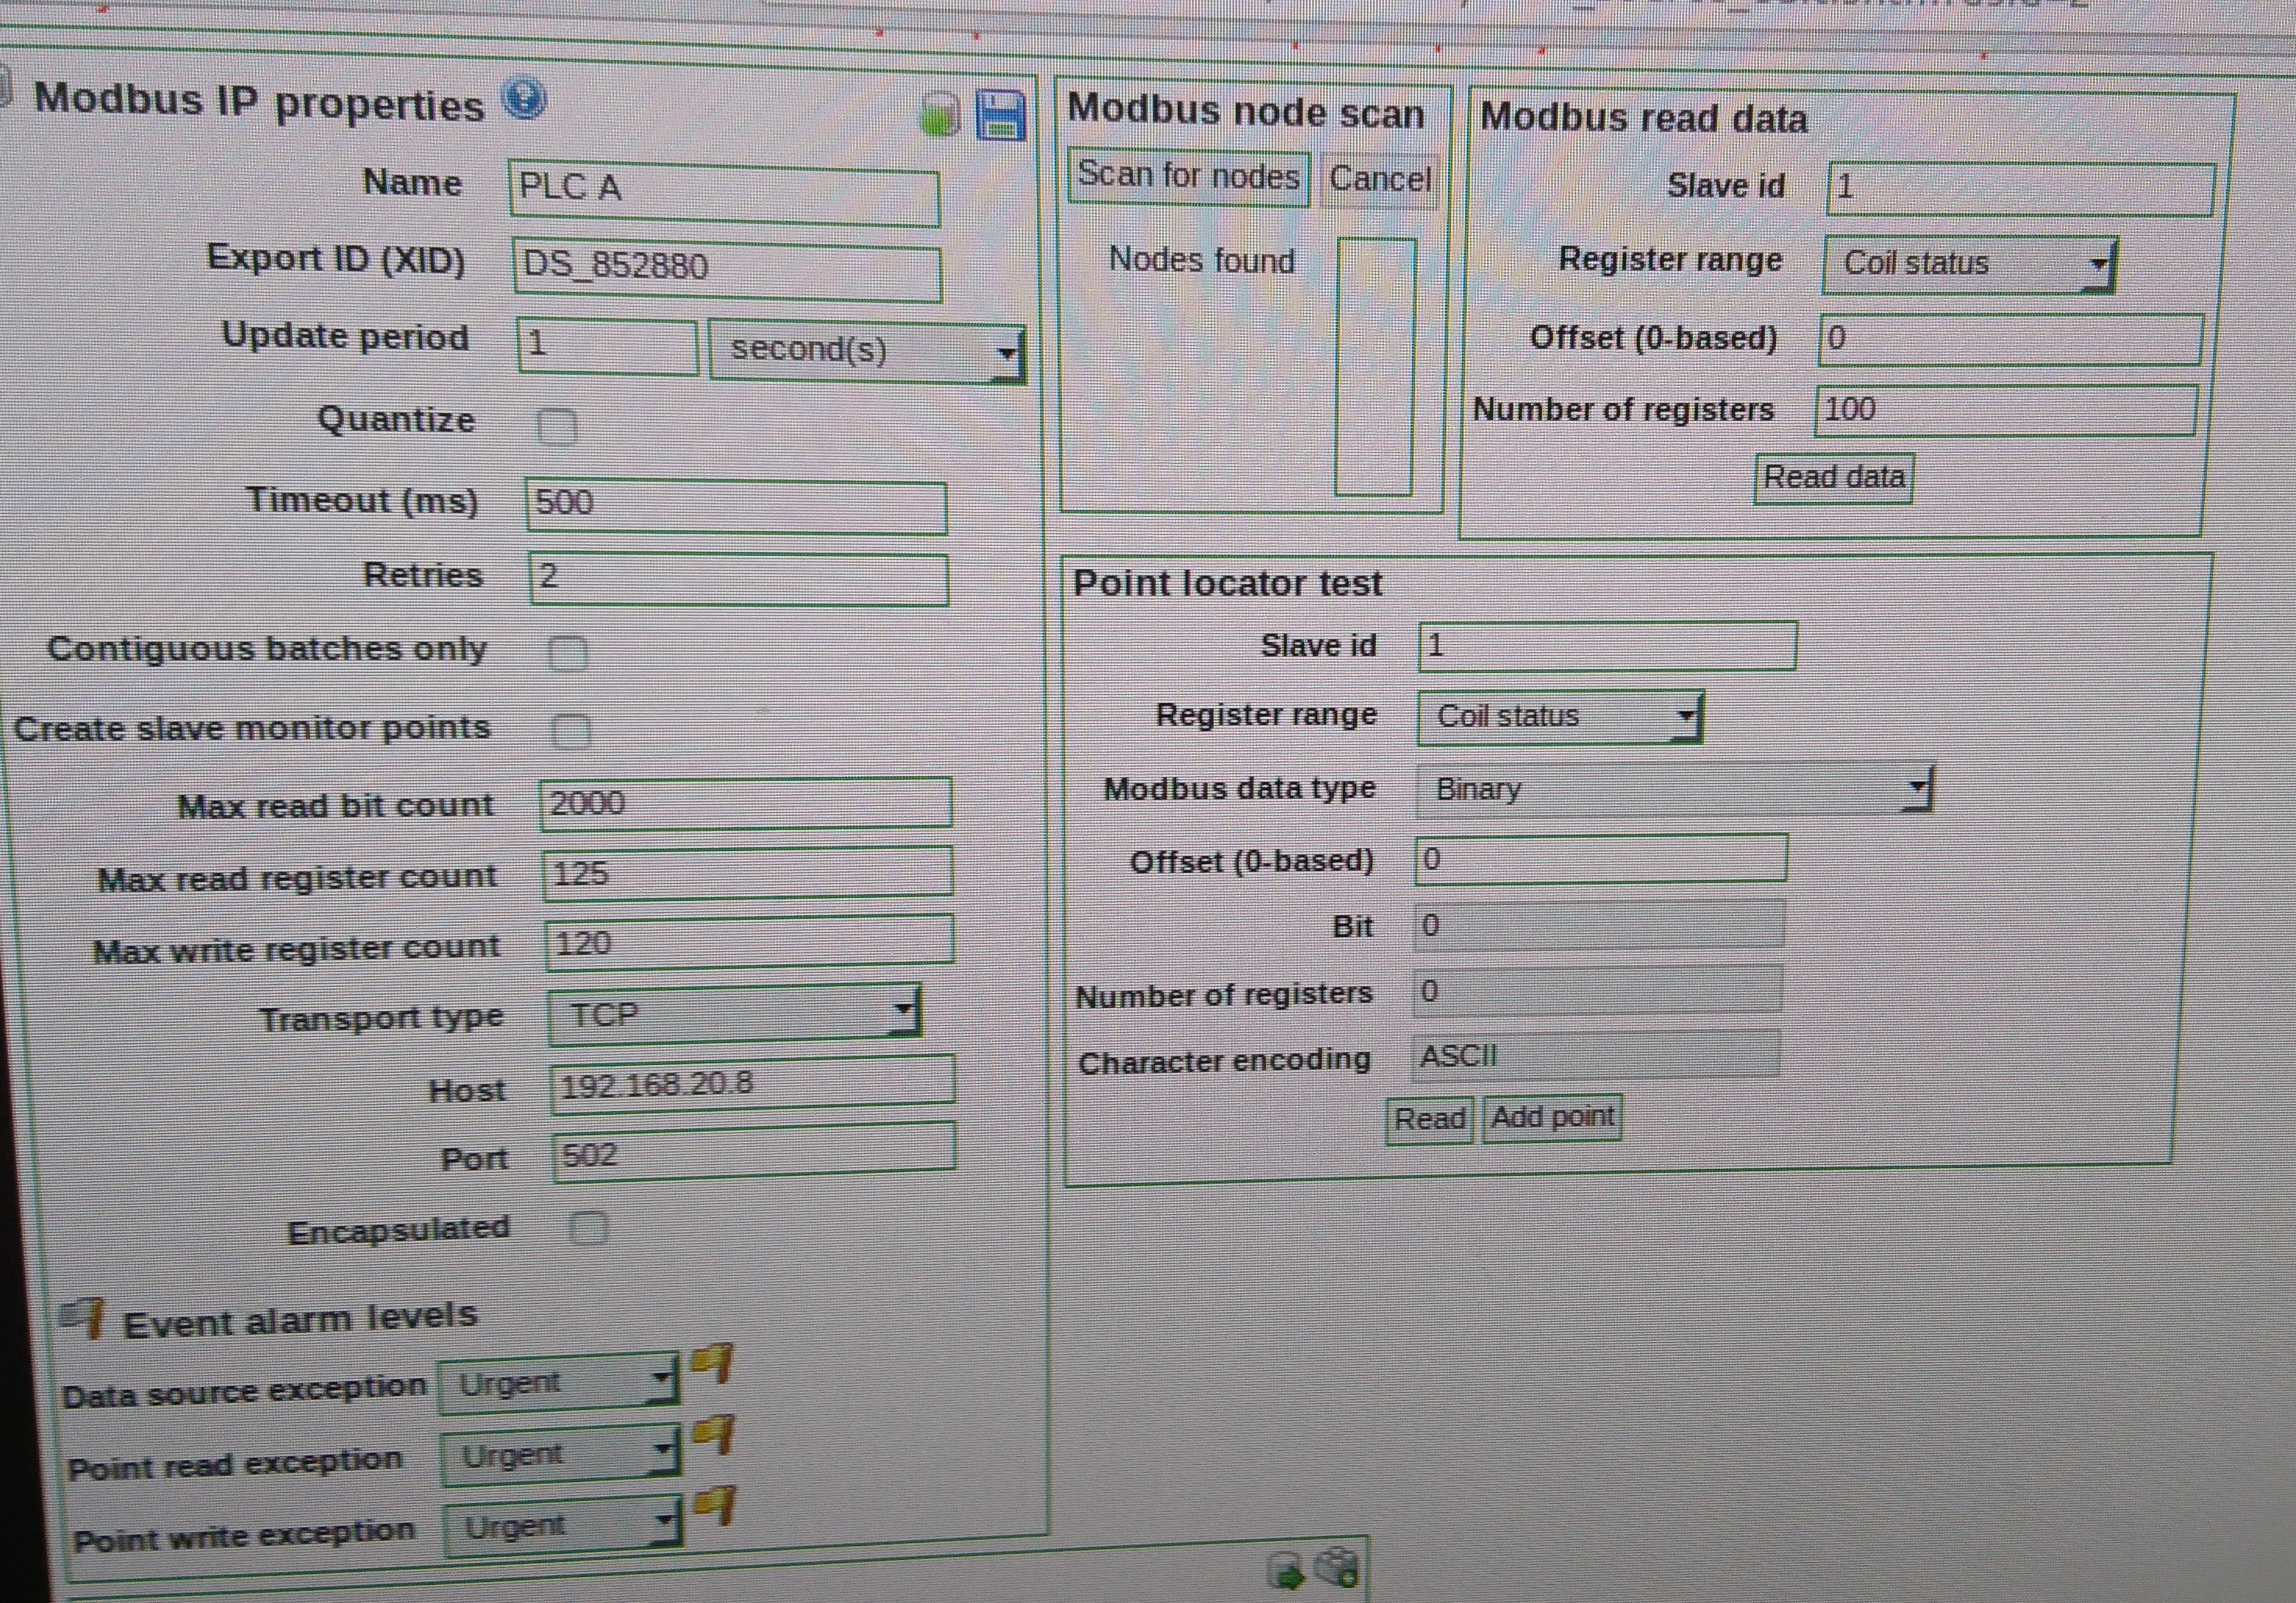
\includegraphics[width=\linewidth]{Figures/ScadaBRplcA.JPG}
		\item Save the new data source
		\item Click on the PLC A's edit button
		\item Under the "Points" section, click the "Add" button to add the following new 'Points'.  \\
		\begin{tabularx}{\linewidth}{*6{| >{\centering\arraybackslash}X}@{}|}
			\hline
			\textbf{Name} & \textbf{Data Type} & \textbf{Status}  & \textbf{Range} & \textbf{Offset} & \textbf{Settable} \\ \hline
			auto & Binary & Enabled & Coil status & 2 & Y \\ \hline
			pump & Binary & Enabled & Coil status & 1 & Y \\ \hline
			valve & Binary & Enabled & Coil status & 0 & Y \\ \hline
			water\_level & 2-byte Signed Int & Enabled & Holding register & 0 & Y \\ \hline
		\end{tabularx}
		\item Repeat the previous steps for PLC B. Use IPv4 address 192.168.20.9. Add the following points to PLC B.\\
		\begin{tabularx}{\linewidth}{*6{| >{\centering\arraybackslash}X}@{}|}
			\hline
			\textbf{Name} & \textbf{Data Type} & \textbf{Status}  & \textbf{Range} & \textbf{Offset} & \textbf{Settable} \\ \hline
			chlorine\_lvl & 2-byte Signed Int & Enabled & Holding register & 1 & Y \\ \hline
			chlorine\_ppm & 2-byte Signed Int & Enabled & Holding register & 2 & Y \\ \hline
			in\_valve & Binary & Enabled & Coil status & 0 & Y \\ \hline
			ou\_valve & Binary & Enabled & Coil status & 1 & Y \\ \hline
			pump & Binary & Enabled & Coil status & 2 & Y \\ \hline
			water\_level & 2-byte Signed Int & Enabled & Holding register & 0 & Y \\ \hline
		\end{tabularx}
		\item Navigate to the "Graphical views" section. Click on "new view"
		\item Create a view that looks like this: \\
		\includegraphics[width=\linewidth]{Figures/HMI.JPG}
	\een
	\item Create the Windows Enterprise and Engineering Workstations
	\ben
		\item Download the Windows 10 VM from \url{https://developer.microsoft.com/en-us/windows/downloads/virtual-machines}
		\item Open the VM using virtualization software of your choice. Follow the on-screen prompts.
		\item Power on the Windows 10 VM
		\item In your virtualization software, add a single NIC to the Windows 10 machine that is connected to the following vSwitch Network: Enterpise (if the Enterpise WS) or ICS (if the Engineering WS)
		\item Repeat for both Windows 10 Work Stations
	\een
	\item Network the Windows Workstation machines (Set the IP Addresses as defined in the \hyperref[fig:netDiagram]{network diagram})
	\ben
		\item Log onto one of the Windows Workstations
		\item In the search bar, search for "Network and Sharing Center". Press ENTER.
		\item Click on "Change Adapter Settings" on the left-hand side of the "Network and Sharing Center" window.
		\item On the "Network Connections" windows, right click on the intended network interface and select "Properties" in the pull-down menu.
		\item Select "Internet Protocol Version 4(TCP/IPv4) Properties". On the "General" tab, select the radio button "Use the following IP Address:"
		\item Enter the appropriate IP address in the "IP Address" field
		\item For the Engineering WS, Enter 192.168.10.1 in the "Gateway" field\\
		For the Enterprise WS, Enter 192.168.100.1 in the "Gateway" field
		\item Repeat for both Windows 10 Work Stations
	\een
	\item Create Windows 2012 Server
	\ben
		\item Download the Windows 2012 R2 Server from \url{https://www.microsoft.com/en-us/evalcenter/evaluate-windows-server-2012-r2}. Select the ISO file.
		\item Follow the on-screen installation instructions for creating a new VM in your virtualization platform.
		\item In your virtualization software, add a single NIC to the Windows 2012 Server machine that is connected to the Enterprise vSwitch.
	\een
	\item Configure the Windows 2012 Server
	\ben
		\item After successful installation of Windows Server 2012, set the IP Address using the same method described for the Windows 10 Workstations. Once again, the appropriate IPv4 address is described in the \hyperref[fig:netDiagram]{network diagram}. In this case, it is address 192.168.100.25.
		\item Install DNS and Active Directory services on the machine.
		\ben
			\item Boot the VM and log on to the server.
			\item Open "Server Manager" and click on the "Dashboard". Click on "Manage" in the top-right corner.
			\item Select "Add Roles and Features". Click on "Next". 
			\item Click on "Role-based or feature-based installation" radio button and click "next".
			\item Select this server as the destination server. Click "next".
			\item Check the boxes for "Active Directory Domain Services" and "DNS Server" in the list. Click "next".
			\item Click on next two more times.
			\item Check the "Restart destination server automatically if required" box and click "Install".
			\item After restarting, open "Server Manager" and click on the flag icon in the upper right.
			\item Select "Promote this server to a domain controller".
			\item Click on the "Active Directory Domain Services Configuration Wizard". Add a new forest called, "radicl.security". Click "Next".
			\item Follow the rest of the on-screen prompts using default configurations until the machine restarts.
		\een
	\een
	\item Add the Windows Workstations to Domain
	\ben
		\item Log-on to the Windows 10 Workstations.
		\item In the search bar, type in "System".
		\item Click "Change settings".
		\item On the "System Properties" window click on "Change...".
		\item On the "Change Name/Domain Changes" window select the "Domain" radio button under "Member of".
		\item Type into the field "radicl.security" and click "ok".
		\item Reboot the system for the changes to take affect.
		\item Repeat for the other Windows Workstation.
	\een
	\item Create pfSense VM
	\ben
		\item Download the ISO file from \url{https://www.pfsense.org/download/}. Follow the on screen instructions for installing the pfSense OS on your VM.
		\item In your virtualization software, add two NICs to the pfSense VM. One should be connected to the "Enterpise" vSwitch and one to the "ICS" vSwitch.
	\een
	\item Configure pfSense
	\ben
		\item On the pfSense machine, choose option "1) Assign Interfaces"
		\ben
			\item Assign WAN to the "Enterprise Network" interface
			\item Assign LAN to the "ICS Network" interface
		\een
		\item Choose option "2) Set interface(s) IP address"
		\ben
			\item Set the WAN IPv4 address to: 192.168.100.1/24
			\item Set the LAN IPv4 address to: 192.168.10.1/24
		\een
		\item Log onto the Engineering Workstation (Windows 10)
		\item Open the web browser and navigate to "192.168.10.1"
		\item Log into pfSense (default credentials)
		\item Navigate to "Firewall/LAN/rules"
		\item Add an "any-any" firewall rule. This will also the enterprise machines to connect to the ICS network. This will give students a chance to add more secure firewall rules later.
		\item The LAN network should already have an "any any" rule. If not, add it.
		\item Remember to click "Apply changes"
	\een
\een

\textbf{Test Network Configuration}\\
\ben
	\item Log onto the pfSense machine.
	\item Choose the option "7) Ping host"
	\item Ping each machine on the "Enterprise network".
	\item If there is a ping failure check the following:
	\ben
		\item The machine being pinged is ON
		\item The machine being pinged has the appropriate IPv4 address
		\item pfSense has the appropriate IPv4 addresses
		\item Ensure there is not a conflicting firewall rule. (Both networks should have "any any" rules)
	\een
	\item Ping each machine on the "ICS network"
	\item Log onto the OpenPLC A machine
	\item Open a shell
	\item Ping OpenPLC B and the I/O Ubuntu machine
\een

\textbf{Starting the Testbed}\\
\ben
	\item Log onto each PLC and do the following
	\ben
		\item Open a terminal
		\item Enter the command: \textit{cd OpenPLC\_v3/webserver/}
		\item Run the OpenPLC runtime with \textit{sudo python ./webserver.py}
	\een
	\item Log onto the I/O Ubuntu machine
	\item Open a terminal
	\item Enter the command: \textit{cd Desktop/Hardware\ Emulation/}
	\item Run the I/O simulation: \textit{sudo python vWaterLab.emu.py}
\een

%-----------------------------------------------------------------------------------------------------------------------------------------------------------------------------------------------------------------%
\pagebreak
\textbf{Change Log}\\\\

\begin{tabularx}{\linewidth}{*3{| >{\centering\arraybackslash}X}@{}|}
	\hline
	\textbf{Change(s)} & \textbf{Contributor(s)} & \textbf{Effective Date} \\ \hline
	First draft of the tutorial & Matthew Kirkland & March 3rd, 2019 \\ \hline
	Second draft of the tutorial & Matthew Kirkland & May 1st, 2019 \\ \hline
	Added Setup of vWaterLab & Matthew Kirkland & May 12th, 2019 \\ \hline
\end{tabularx}

%-----------------------------------------------------------------------------------------------------------------------------------------------------------------------------------------------------------------%
\pagebreak

% this style of bibliography shows urls
\bibliographystyle{IEEEtran}
\bibliography{bibliography}{}

\end{document}